\section{Placement and Routing (WIP)} \label{sec:mapping}
\if 0
\subsection{Back-tracking + A* search Placement and Routing}
\begin{figure}[!ht]
  \small
  \begin{description}
    %\item [var] BG: weighted bipartite graph containing mapping of $bs \leftrightarrow ps$
    %$BG.V$ and $BG.P$ are unmatched $v$s and $p$s in $BG$. 
    %$BG.w[p,v]$ is the weight between $p$ and $v$, relates to the cost to match $v$ to $p$.
      %Initially all weights are equally assigned.
    %\item [function] \textsc{isValid}(BG):
      %$\forall v in BG, |BG[v]| \neq 0$
    %\item [var] R: data structure keeping track of routes between ps
    %\item [function] \textsc{map}(BG,v,p): 
      %Remove all edges in BG connected with v and p except between v and p. The function can fail if
      %resulting BG has p with no edge
    \item [function] \textsc{advance}($BG,v,p$):
      Perform a single step walk the PB graph, where reached $p$ can be a switch, router, or a terminal.
      Return reached $ps$ and their costs.
    \item [function] \textsc{search}($BG,p1,p2$):
      Find the shortest path between $p1$ and $p2$ using A* search. Use \textsc{advance} function to walk
      the PB graph and get cost of each step. Return route with minimum total cost. The function can
      fail if no possible route exists between $p1$ and $p2$
    \item [function] \textsc{span}($BG,v,p$):
      Similar to search except without a destination. Find all $ps$ (must be end node, cannot be a router or switch) reached by 
      walking the PB graph and returning cost of each reached $p$.
    %\item [function] \textsc{rankV}(BG,v):
      %($-|BG[v]|$, $\sum BG.w[v,p] \forall p \in BG[v]$)
    %\item [function] \textsc{rankP}(BG,v,p):
      %($-BG.w[v,p], -|BG[p]|$)
  \end{description}

  \raggedleft
  \begin{algorithmic}
  \Function{match}{$BG$}
    \algnotext{EndFor}
    \algnotext{EndIf}
    \If { $\Call{isMached}{BG,p} \forall p \in BG }$ \Return BG \EndIf 
    \For { $v \gets arg \max_{v \in BG.V} \Call{rankV}{BG,v}$ }
      \For { $p \gets arg \max_{p \in P} \Call{rankP}{BG,v,p}$ }
         \State $BG' \gets \Call{map}{BG, v, p}$ *
         \If { !\Call{isValid}{$BG'$} } {\bf continue} \EndIf
         \State $reached, costmap \gets span(BG',v)$
         \For { $nv \in \Call{neighbor}{v}$ }
            \If {$\Call{isMatched}{BG,nv}$}
              \State $np \gets BG'[nv]$
              \State $BG'.R[p,np] \gets \Call{search}{BG',p,np}$ *
            \Else
              \State $BG'[nv] \gets BG'[nv] \cap reached$ *
              \For { $np \in BG'[nv]$ }
                \State $BG'.w[nv,np] += \frac { costmap[np] }{ \Call{degree}{p}} $
              \EndFor
            \EndIf
        \EndFor
        \If {\Call{isValid}{$BG'$}} {\bf continue} \EndIf
        \State $BG', R' \gets \Call{match}{BG',R'}$ *
        \If {\Call{isValid}{$BG'$}} {\bf continue} \EndIf
        \State \Return $BG', R'$
      \EndFor
    \EndFor
    \State \Return Failed in matching
  \EndFunction
  \end{algorithmic}
  \caption{Backtracking + A* search placement and routing (* statements can cause backtracking).}
  \label{alg:backtrack}
\end{figure}

Figure \ref{alg:backtrack} shows the algorithm to perform back-tracking matching with look-ahead on the initial
placement. The algorithm starts with the weighted bipartite graph ($BG$) after resource pruning, and iteratively
places and routes all the VBs. Weights in $BG.w[w,p]$ indicates the cost to map $v$ to $p$ and are initialized to be
equal. $BG.R$ stores the routing between any two PBs. A $BG$ is valid if all of its VBs have at least an edge to a PB.
When mapping a $p$ to $v$, all edges connected to them except between them are removed. 

At each step of the matching, the algorithm starts with the most ``difficult'' VB $v$, measured by
{\sc rankP}. {\sc rankP} is a function inversely proportional to the number of choice of PB ($|BG[v]|$)
and proportional to sum of the cost of its choices ($\sum BG.w[v,p] \forall p \in BG[v]$).
Then it picks a $p$ with the smallest cost in $BG.w[v,p]$, and, if there is more than one, the one with the fewest choices of VB ($|BG[p]|$). 
%The intuition for the second term is to encourage specialized PBs to be used on the special VBs.
Then, the algorithm tries to match $v$ to $p$. The {\sc map} function will fail if mapping $v$ to $p$ causes other $v'$ to be unmatchable. 
Next, the {\sc span} function finds all reachable $p'$s from the current $p$ and return
a cost map for each reached $p'$. 

Then, the algorithm loops through each neighbor $nv$ of $v$ in VB
data-flow graph. If the neighbor is already matched, it tries to route all connections between $v$
and $nv$ by finding shortest path between $p$ and $BG[nv]$ using A* search. Otherwise, $v$
constrains
neighbor $nv$'s choice to be intersection of $nv$'s original choice and reachable $p$s from the {\sc
span}. Next, weights of the pruned choices $BG.w[nv,np] \forall np \in BG[nv]$ are added with a new cost.
The new cost is computed as the cost to walk from $p$ to $np$ divided by degree of the $v$. This step ``forecasts'' the cost of mapping $nv$ to $np$ in the future by aggregating the current cost from $p$ to $np$. 

Then, if $nv$ has multiple neighbors, all neighbors will accumulate their predictions of the further costs to $nv$'s choices. The division factor
is to reduce the penalty of broadcast links such that they are allowed to travel further. If all
$*$ statements in Figure \ref{alg:backtrack} succeed, which means all $v$ in $BG$ has at least a
choice, the algorithm proceed on {\sc match} the next $v$. If the {\sc match} succeed, return the
new $BG$, otherwise try the next $p$ or $v$ with highest rank.

By starting with the most difficult $v$ to match, the algorithm is able to quickly prune the search space.
By constraining and aggregate costs to its neighbors, $v$'s neighbors becomes more difficult to map. As a
result, the algorithm tends to map $v$s topologically based on VB data-flow graph, which optimizes
for adjacency between $v$s. 
\fi
%At high-level, the algorithm starts with the most difficult $v$ to match, which are usually the ones that are
%specialized such as the ones connected to DRAM interface. Next, the algorithm look-ahead on future high cost $p$s for its neighbor by adding the cost from its current location $p$ to those $p$s of the neighbors. This is the key step to prune the search space for backtracking, which allows worst design to place and route in within 15min.
%By constraining and aggregate costs to
%its neighbors, $v$'s neighbors becomes more difficult to map. As a
%result, the algorithm tends to map $v$s topologically based on VB data-flow graph, which optimizes
%for adjacency between $v$s. Furthermore, the {\sc span} and {\sc search} function takes in another
%function {\sc advance}, which is a function that returns a list of next-hop physical nodes and their
%costs as walking on the PB graph. The cost returned by {\sc span} and {\sc search} is simply
%sum of costs from each hop. The physical nodes in {\sc advance} can includes intermediate
%physical transit
%nodes such as routers for dynamic network and switches for static network, while {\sc span} only
%returns terminal PBs. {\sc advance} also takes
%in $BG$ as input, which for static network, preventing walking on physical links that are already 
%occupied. For dynamic network, the cost of walking on a link is proportional to the number of times
%the link is utilized, which allows but penalizes link sharing. This algorithm is topology
%agnostic, where the only topology specific function is {\sc advance}. The cost returned by {\sc advance}
%also incorporates a topology dependent heuristic cost to speed up A* search. An example heuristic cost
%for mesh network is the Manhattan distance between the next hop to the final destination.

%\subsection{Iterative Placement}

For purely static networks, the goal is primarily to find a valid placement---because static routes have guaranteed resources reserved, no two routes can conflict, and any placement found is essentially optimal. 
Some routes may have longer latency, which has a second-order performance impact compared to throughput.
However, determining a purely static allocation of routes cannot be done in polynomial time and may be infeasible; therefore, the static network must be over-provisioned to aid placement.
Although virtually all placements are valid for the dynamic and hybrid networks,
not all valid placements are equal---some have less congestion and therefore run several times faster.
%\info{this sentence is a bit confusing and not exactly true. Static routes can have different latencies and can also 
%change program performance. It's just a second order cost compared to throughput. The potentially confusing part is that
%if it's optimal then why would the placer do work at all}
%For a static network, it is impossible for two routes to interfere with each other: they have guaranteed resources reserved, so the placement can stop as soon as a satisfying assignment of routes is found.

%Therefore, the dynamic network placement is performed with an iterative algorithm that uses heuristics (summarized in Table~\ref{tab:heur}) to rapidly evaluate placements; the algorithm is summarized in Figure~\ref{alg:place}.
Dynamic network placement is performed with an iterative algorithm using heuristics to rapidly evaluate placements: a penalty score is assigned as a linear function of several subscores.
These include projected congestion on dynamic links, projected congestion at network injection and ejection ports, the average route length, and the length of the longest route.
We estimate congestion by normalizing the number of packets on each link to the program link with the highest total packet count.
The most active program link sets a lower bound on the program runtime (the highest bandwidth physical link can still only send one packet per cycle), which translates to an upper bound on congestion for other links.
%, under the assumption that at least one pipeline in the design is almost always active.
We start with random placement of the VBs.
Then, a genetic algorithm shuffles the VBs whose links contribute most to congestion, and keeps the new position if it improves the route assignment.
By iteratively re-placing and re-routing, the mapping process eventually converges to a good placement.
%Then, the most congested injection port, ejection port, or network link is found, and its packet count is normalized to the ideal number of clock cycles.
%\begin{table}
%  \centering
%  \begin{tabular}{r|l}
%    Weight & Description\\\hline
%%           & Worst injection port flits* \\
%%           & Worst ejection port flits* \\
%%           & Worst link flits* \\
%           & Estimated network slowdown\\
%           & Longest overall route (hops) \\
%           & Weighted average hops \\
%  \end{tabular}
%  %\caption{The penalty heuristics used by the dynamic placement algorithm. Values marked with * are normalized to the theoretical optimal cycle count.}
%  \caption{The penalty heuristics used by the dynamic placement algorithm.}
%  \label{tab:heur}
%\end{table}

%\begin{figure}
  %\centering
  %\small
  %\begin{algorithmic}
%
%  \Function{RouteValiant}{$cand, route$}
%    \Function{ScoreValiant}{$cand, route$}
%      \State $cong \gets 0$
%      \State $static \gets 1000$
%      \ForAll{$hop \in route$}
%        \State $cong \gets \max(cong, cand[hop].cong)$
%        \State $static \gets static \land cand[hop].static < lim$
%      \EndFor
%      \State \Return $cong+static$
%    \EndFunction
%    \State $opt\gets route_\infty$
%    \ForAll{$int\_hop$ in $route$}
%      \ForAll{${first,second} \in \{XY,YX\}$}
%        \State $test\_route\gets route\_dor(first, route.begin, int\_hop) + route\_dor(second, int\_hop, route.second)$
%        \If {$ScoreVal(test\_route) < ScoreVal(opt)$}
%          \State $opt \gets test\_route$
%        \EndIf
%      \EndFor
%    \EndFor
%    \State \Return $opt$
%  \EndFunction
%  \Statex
  %\Function{RouteDijkstra}{$cand, src, dsts$}
    %\Function{HopWeight}{$cand, hop$}
      %\If{$cand[hop].static < lim$} \State \Return $1$ \Else \State \Return $100*cand[hop].cong$ \EndIf
    %\EndFunction
    %\State $prog\_edges \gets \{\}$
    %\ForAll{$A,B \in \{src, dsts\}, A \neq B$}
      %%\State $prog\_edges \gets \{prog\_edges, \Call{ShortestPath}{A, B, HopWeight}\}$
      %\State $prog\_edges \gets \{prog\_edges, \Call{MinPathWeighted}{A, B}\}$
    %\EndFor
    %\State $reached \gets \{src\}$
    %\State $remaining \gets dsts$
    %\State $route \gets \{\}$
    %\While {$remaining$} 
      %\State $min \gets edge_\infty$
      %\ForAll{$E \in prog\_edges$}
        %\If{$E.src \in reached \land E.dst \in remaining \land E.weight < min$}
          %\State $min \gets E$
        %\EndIf
      %\EndFor
      %\State $remaining \gets remaining \setminus min$
      %\State $reached \gets reached \cup min.src$
      %\State $route \gets route \cup min.hop$
    %\EndWhile
    %\State \Return $route$
  %\EndFunction
  %\end{algorithmic}
  %\caption{The routing algorithms.}
  %\label{alg:route}
%\end{figure}
%
%\begin{figure}
%  \centering
%  \small
%  \begin{algorithmic}
%
%  \State $pool \gets \Call{Initialize}{VBGraph, PBGraph}$
%  \For{$i \gets 1,it$}
%    \ForAll{$cand \in pool$}
%      \If{$\neg \Call{Frozen}{cand}$}
%        \State $cand \gets \Call{unplace}{cand}$
%        \State $cand \gets \Call{Place}{cand}$
%        \State $cand \gets \Call{Route}{cand}$
%        \State $cand \gets \Call{Score}{cand}$
%      \EndIf
%    \EndFor
%    \State $pool \gets \Call{Filter}{pool}$
%  \EndFor 
%  \State \Return $\Call{Best}{pool}$
%  \end{algorithmic}
%  \caption{The iterative re-placement algorithm.}
%  \label{alg:place}
%\end{figure}

%The {\sc Unplace} function randomly decides between unplacing a random node, and unplacing one or several nodes based on heuristics.
%For the heuristic based unplacement, a node's contribution to global route congestion is calculated by adding an estimate of all connected routes' contributions to the global penalty score; the node(s) with the highest scores are unplaced.
%Similarly, {\sc Place} also can either randomly place an unplaced node, or place it to minimize the Manhattan distance to its logical neighbors. {\sc Score} calculates the heuristics for each node, and {\sc Filter} duplicates the best candidate placements to fill the pool. Because the unplacement and replacement steps can make a placement worse, the best performing placements are frozen in each iteration to ensure that no good placements are thrown away.

\subsection{Congestion-aware routing}
%\info{Somewhere we should mention that placement and routing running interchangeably}
To achieve optimal performance, we use a routing algorithm that detects congestion and routes around it. 
Routing starts with the highest-priority routes, as determined by fanout and activation count, which are fixed after they are routed.
This makes sure that the static network is used most efficiently.
%
Our scheme searches a large space of routes for each link, using Dijkstra's algorithm \cite{dijkstra} and a hop weighting function.
Routes are not analyzed on the basis of a single source-destination pair, which would be inadequate for broadcasts: instead, a directed graph is built from the source and all destinations in the route, with edge weights corresponding to the minimal route between each pair of VBs in the broadcast.
For example, if the broadcast is from VB-1 to VB-2 and VB-3, four total potential routes are analyzed for congestion: VB-1 to VB-2, VB-1 to VB-3, VB-2 to VB-3, and VB-3 to VB-2.
The routes are weighted so that routes mapped on the static network are preferable to those mapped to the dynamic network; within these categories, routes are weighted based on length. 

%\info{does the nodes refers to only source and destinations or including all nodes on the path between source and destination. How does the weights represent the minimum routes? Is it capturing the cost of minimum route?}
Then, a search algorithm based on Prim's algorithm for minimum spanning trees \cite{prim1957shortest} is run to build a tree for the broadcast, starting with only the source being reached.
At every step, the most-preferable route (from the graph built using Dijkstra's algorithm) that adds a new destination VB to the reached set is chosen and added to the broadcast, until all destination VBs are reached. 
This route can start from either the source of the broadcast tree or any destination currently in the reached set.
The algorithm will find a fully static broadcast tree, if one exists, and will only add a non-static route to the broadcast (moving the entire broadcast to the dynamic network) when there are VBs in the tree that cannot be reached from the source VB by \emph{any} static route.
%\info{does the algorithm routes links from high priority to low from all nodes or it does one node at a time?}

\subsection{VC allocation for deadlock avoidance} \label{sec:vc_alloc}
Deadlock is a system pathology in dynamic routing where multiple flits form a cyclic holds/waits dependency on each others' buffers and prevent forward progress.
Most data-flow accelerators use a streaming model, where outputs of a producer are sent over the network to one or more consumers
without an explicit request; the producer is backpressured when there is insufficient buffer space. 
While this paradigm improves accelerator throughout by avoiding the round-trip delay of a request-response protocol, it introduces an additional source of deadlock \cite{hansson2007avoiding}. 

Figure~\ref{fig:deadlock}(a) shows a sample VB data-flow graph, which is statically placed and routed on a $2\times3$ network in (b). 
Logical links B and C share a physical link in the network. If C fills the buffer shared with B, VB-3 will never receive any packets from B and will not make forward progress.
%For y-z dimension-order routing, the only valid routes from VB-1 to VB-3 is through $\[0,1\], \[0,0\], \[1,0\], \[2,0\]$. 
%Dimension-order routing prevents deadlock by eliminating cycles in network routes.
%On traditional NoCs, deadlock can be solved with dimension-order routing, which routes all traffic on one dimension before another.
%\yaqi{
  With streaming computation, the program graph must be considered as part of the network dependency graph, which must be cycle-free to guarantee deadlock freedom. However, this is infeasible because cycles can exist in a valid VB dataflow graph when the original program has a loop-carried dependency. Therefore, deadlock avoidance using cycle-free routing, such as dimension-order routing, does not work in our scenario. 
Allocating VCs to prevent multiple logical links from sharing the same physical buffer is consequently the most practical option for deadlock avoidance on streaming accelerators.
%Because the entire program is connected through these streaming dependencies, any two links can conflict and result in a deadlock.
%\yaqi{However, cycles are permitted in the programming paradigms since loop-carried dependencies can be mapped across the network.
%Therefore, we perform VC allocation at each router to prevent multiple logical links from sharing the same physical buffer.
\if 0
Virtual channel (VC) allocation is another common approach to avoid deadlock. We can statically assign conflicting streams B and C with different
virtual channels at router $[2,0]$, which prevents them to share physical buffers. 
Notice indirect inputs of a VB, such as A and D with eventual consumer VB-3,
also need distinct VCs to ensure deadlock-free. To minimize the number of VCs required, we perform per-hop VC allocation--statically
assign conflicting links at each input of each router with distinct VCs. The VCs can be looked up at runtime based on link ID.
Distinct links from the same source VB, such as A and C, can share the same VC, because VB-1 ensures the number of flits sent over A and C remains
to a ratio that receiver expects, which permits data to drain in the network.
\fi

\begin{figure}
\centering
\includegraphics[width=0.7\columnwidth]{figs/deadlock.pdf}
  \caption{An example of deadlock in a streaming accelerator, showing the (a) VB data-flow graph and (b) physical placement and routes on a $2\times3$ network. There are input buffers at all router inputs, but only the buffer of interest is shown.}\small\textsuperscript{}\label{fig:deadlock}
\end{figure}

%Deadlock is a system pathology that occurs when multiple actors hold resources while waiting for each other's resources to become available.
%In a NoC, the actors are flits, and the held/waited-for resources are buffers.
%There are four necessary conditions for permament deadlock \cite{coffman1971system}:
%\begin{enumerate}
%  \item resources are mutually exclusive,
%  \item actors hold resources while waiting on other resources,
%  \item actors can not be preempted, and
%  \item actors wait on each other in a cyclic graph.
%\end{enumerate}

%In traditional NoC designs, there are two types of deadlock: deadlock within a network (such as that from cyclic paths), and \emph{protocol deadlock}.
%These designs are typically based around a request-response model: to avoid protocol deadlock, a node issuing a request will always be ready to receive its response. 
%Then, to ensure that the protocol graph is acyclic, the responses are prevented from waiting indefinitely on resources held by requests by partitioning all buffers in the network into two classes.
%Deadlock within a network is avoided by a variety of schemes, many of which (dateline VC allocation, dimension-order routing) work by imposing restrictions on which holds/waits relationships are valid.
%These restrictions ensure that the full potential holds/waits graph is acyclic, and therefore any subgraph must also be acyclic.

%When extending the deadlock model to a CGRA, there are three main types of deadlock that we need to avoid: traditional network deadlock, endpoint buffer deadlock, and through-node deadlock.
%For CGRAs, there are three main types of deadlock that we need to avoid: traditional network deadlock, endpoint buffer deadlock, and through-node deadlock.
%The key difference between CGRA and CPU networks is that CGRAs operate in a streaming fashion---each spatially distributed node, after completing its assigned work, sends the result to the next node(s).
%Furthermore, each node has fixed-size input buffers which, with the long distances possible between nodes, are far too small to perform high-throughput end to end credit-based flow control \cite{wang2013avoiding}.
%Finally, nodes propagate backpressure signals from their outputs to their inputs, which means that they must be considered as part of the network graph \cite{hansson2007avoiding}.
%This is similar to work done on streaming NoCs, where multiple streams of traffic compete for the same resources \cite{hansson2007avoiding, wang2013avoiding}.
%\begin{figure}
  %\centering
  %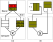
\includegraphics[width=0.4\columnwidth]{figs/deadlock_figs.pdf}
  %\caption{Two forms of network deadlock for CGRA dynamic networks. The left shows input buffer starvation, and the right shows a packet taking an ``illegal'' turn through a node.}
  %\label{fig:deadlock}
%\end{figure}
%Furthermore, because a compute node must be able to send its output to read its inputs, dependences may be propagated backwards through the network; this means that dimension order routing alone is insufficient to make progress and separate virtual networks must be used.
%\subsection{Endpoint Buffer Deadlock}
%This is a type of protocol deadlock that results from head-of-line blocking and finite buffer sizes at node inputs, as shown in Figure~\ref{fig:deadlock}(a).
%Consider two streams, A and B, that traverse the same virtual channel but are destined for different input buffers at the same destination node.
%If A fills up its input buffer, and B's input buffer is empty, the node cannot make progress.
%Simultaneously, if a flit from stream A is at the head of the shared virtual channel, then no flits from stream B will be able to pass it.
%
%At the final hop of the network, this would be trivial to resolve: the final router can use its knowledge of the buffer state of the destination to avoid overloading any single input buffer.
%However, it could be too late to resolve this problem at the final router, because if it blocks the faster flow, and they share a network resource earlier, the slower flow could be head-of-line blocked earlier in the network.
%\subsection{Through-Node Deadlock}
%Because nodes do not have infinite buffers, the deadlock graph for a network no longer begins and ends at the routes---it must be extended with information about the program nodes \cite{hansson2007avoiding}.
%%This means that traditional deadlock avoidance techniques, such as dimension-order routing, are \emph{not sufficient} to prevent deadlock in these networks.
%An example of how this can cause deadlock in a y-first dimension-order routed network is shown in Figure~\ref{fig:deadlock}(b).
%This type of deadlock can also combine with endpoint deadlock, in addition to traditional network deadlock.
%Because nodes propagate holds/waits dependences, any indirect input to the final node is capable of creating an endpoint buffer deadlock at the final node with any other indirect input, anywhere in the network.
%When different branches of the tree are fed by different DRAM accesses, one will almost certainly run faster and inevitably lead to this deadlock condition.
%Practically, this means that no two logical paths may be allowed to conflict at \emph{any} point in the network; to meet this guarantee, buffer allocation is performed to ensure that all logical paths traversing the same physical link are placed into separate virtual channels.
%Because there are only a finite number of VCs at each router, this is another network constraint to optimize: routes are penalized for exceeding the maximum, which leads to them being moved and a better solution being found.

%\subsection{Priority VC}
%Although we require up to 2 VCs for efficient place and route, the overall link congestion of the worst dynamic network placement with a parallel vector network is 1---therefore, the majority of these VCs are carrying almost no traffic. 
%Because VC buffers consume the vast majority of dynamic network area, we can save a significant amount of area with a heterogeneous buffering approach.
%One VC, the \emph{priority VC}, is provided with a full-width (512bit) buffer, and the other VCs are provided with smaller (32--64bit) buffers.
%When the placement is generated, each route is analyzed to determine whether it can be allocated entirely in the priority VC; if not, it is split by the sender into 8--16 smaller flits before sending through the network.
%

\section{Simulation (WIP)}
We use a cycle-accurate simulator to model the pipeline and scheduling delay for the two types of architectures,
 integrated with DRAMSim \cite{dramsim} to model DRAM access latency. For static networks, we model
a distance-based delay for both credit-based and per-hop flow control. 
For dynamic networks, we integrate
our simulator with Booksim \cite{jiang2013detailed}, adding support for arbitrary source routing using look-up tables. 
Finally, to support efficient multi-casting in the dynamic network, we modify Booksim to duplicate broadcast packets at the router where their paths diverge.
At the divergence point, the router sends the same flit to multiple output ports over multiple cycles.
We assume each packet carries a unique ID that is used to look up the output port and next VC in a statically generated routing table, and that the ID is roughly the same size as an address.
When the packet size is greater than the flit size, the transmission of a single packet takes multiple cycles.
%\info{is it worth mentioning how large flit are transmitted on small flit routers? are they just treated as packet?}
%We simulate the priority VC functionality by determining which packets will traverse non-priority VCs using the generated placement.
%These packets are scaled, to account for the smaller effective flit size and therefore the need to send multiple flits.

\begin{table*}
\centering
  \footnotesize
  \begin{tabular*}{6.25in}{p{0.75in} p{3in} p{2.5in}}
    \bottomrule
    \textbf{Benchmark} & \textbf{Description} & \textbf{Data Size} \\ \midrule
    DotProduct & Inner product & $1048576$ \\ \midrule
    OuterProduct & Outer product &$1024$ \\ \midrule
    BlackScholes & Option pricing &$1048576$ \\ \midrule
    TPCHQ6 & TPC-H query 6 &$1048576$ \\ \midrule
    Lattice & Lattice regression~\cite{garcia2009lattice} &$1048576$\\ \midrule
    GDA & Gaussian discriminant analysis &$127\times1024$ \\ \midrule
    GEMM & General matrix multiply &$256\times256\times256$ \\ \midrule
    Kmeans & K-means clustering &k=64, dim=64, n=8192, iter=2 \\ \midrule
    LogReg & Logistic regression &$8192\times128$, iter=4\\ \midrule
    SGD & Stochastic gradient descent for a single layer neural network &$16384\times64$, epoch=10 \\ \midrule
    LSTM & Long short term memory recurrent neural network &1 layer, 1024 hidden units, 10 time steps \\ \midrule
    GRU & Gated recurrent unit recurrent neural network &1 layer, 1024 hidden units, 10 time steps \\ \midrule
    LeNet & Convolutional neural network for character recognition& 1 image\\ \midrule
  \end{tabular*}
  \caption{Benchmark summary}
  \label{tab:benchmark}
\end{table*}


\subsection{Area and power}
% Elaborate more here since reviewers were confused
To efficiently evaluate large networks, we start by characterizing the area and power consumption of individual routers and switches
used in various network configurations. 
The total area and energy are then aggregated over all switches and routers in a particular network.
We use router RTL from the Stanford open source NoC router \cite{becker2012efficient} and our own parameterized switch implementation.
We synthesize using Synopsys Design Compiler with a \SI{28}{nm} technology library and clock-gating enabled, meeting timing at a 1 GHz clock frequency.
%For both the switch and the router, we enable clock-gating during synthesis to reduce dynamic power. 
Finally, we use Synopsys PrimeTime to back-annotate RTL signal activity to the post-synthesis switch and router designs to estimate gate-level power.

We found that power consumption can be broken into two types: 
inactive power consumed when switches and routers are at zero-load ($P_{\text{inactive}}$, which includes both dynamic and static power),
and active power. The active power, as shown in Section~\ref{sec:net_char}, is proportional to the amount of
data transmitted. 
Because power scales linearly with the amount of data movement, we model the marginal energy to transmit a single flit of data (flit energy, $E_{\text{flit}}$) by dividing active energy by the number flits transmitted in the testbench:
\begin{equation}
  E_{\text{flit}} = \frac{\left(P-P_{\text{inactive}}\right) T_{\text{testbench}}}{\#\text{flit}} 
\end{equation}
While simulating an end-to-end application, we track the number of flits transmitted at each switch and router in the network, as well as the number of switches and routers allocated by place and route. 
We assume unallocated switches and routers are perfectly power-gated, and do not consume energy.
The total network energy for an application on a given network ($E_{\text{net}}$) can be computed as:
\begin{equation}
  E_{\text{net}} = \sum_{\text{allocated}} P_{\text{inactive}} T_{\text{sim}}
  + E_{\text{flit}}  \#\text{flit},
\end{equation}
where $P_{\text{inactive}},$ $E_{\text{flit}},$ and $\#\text{flit}$ are tabulated separately for each network resource.

%we model the energy needed to transmit a single flit through 
%the designs by using linear regression to separate power consumed when no flits are transmitted (e.g., clock network power) and power consumed when flits are transmitted.
%We assume unused switches and routers can be power gated, and we enable clock gating to reduce dynamic power when network is idle.
%The total network energy of an application on a given network design point is composed of zero-load power for switches and routers that cannot be power gated, and per-flit power for each network communication.

